\documentclass{article}

\usepackage[utf8]{inputenc}

\usepackage{booktabs} 
\usepackage{comment} 
\usepackage{amsmath}
\usepackage{graphicx}
\usepackage{float}
\usepackage{array}
\usepackage{multirow}       % For table multirows
\usepackage[font=small,labelfont=bf]{caption} % For caption formatting


\begin{document}

	\section*{Bibliographical references}
			%small intro and foundational works to have as introduction.test papers.
			Recurrence Quantification Analysis (RQA) and Cross-Recurrence Quantification Analysis (CRQA) are
			nonlinear methods for the analysis of nonstationary time series. 
			%such as EEG signals. 

			The offer the quantification of the recurring patterns in phase space trajectories \cite{trulla1996, webber2005}. 
			Introduced by Trulla et al.\cite{trulla1996} (directly built on quantifying recurrence plots\cite{eckmann1987}) 
			and expanded by Webber and Zbilut\cite{webber2005}, RQA measures metrics 
			like recurrence rate, determinism, and laminarity to capture dynamic system behavior. 
			Thomasson et al.\cite{thomasson2002} in their work, demonstrated RQA’s applicability on EEG data, mentioning 
			the robustness it shows in accordance to noise
			and nonstationarity. Marwan et al.\cite{marwan2013} further advanced recurrence plot techniques,
			emphasizing on developing a confidence measure of RQA in detecting dynamic transitions.
			Works like these, serve as a foundation of applying RQA and CRQA on EEG 
			studies in various conditions such as epilepsy, cognitive disorders and more 
			as explored in this review.

			%ok, eeg OK
			Frolov et al.\cite{frolov} proposed an approach to analyze frequency based multiplex brain networks
			using recurrence quantification analysis (RQA) 
			on EEG data, and demonstrated the way that recurrence-based 
			synchronization indices can effectively capture 
			both within-frequency (intralayer) and cross-frequency (interlayer) 
			functional connectivity during cognitive tasks. 
			Their work showed that RQA is particularly suitable for analyzing 
			non-stationary EEG signals and revealed
			important insights about the evolution of functional connectivity 
			patterns during cognitive tasks. In addition the dataset
			used in this research are openly available in a Figshare repository.

			%ok.   eeg,Alzheimer OK
			Núñez et al. \cite{nunez2020characterization} worked with 
			resting-state EEG recordings from subjects with mild cognitive impairment(MCI), 
			Alzheimer's disease(AD), and healthy ground truth controls in order to detect 
			frequency based changes into their brain dynamics. 
			By blending wavelet based Kullback–Leibler divergence
			(KLD) for capturing non-stationarity,
			and two RQA
			metrics(\textit{entropy of the recurrence point density}
			and the \textit{median of the recurrence point density}) insights have been
			extracted related to neurodegeneration presence.
			Research's findings show that MCI and AD are presenting notable changes in 
			the recurrence structure and non-stationarity of EEG signals,
			and more specifics on the theta and beta frequency bands.
			Therefore, recurrence based dynamics show a capability as potential 
			biomarkers for monitoring and detecting early Alzheimer's disease and its progression.

			%% EEG, RQA-CRQA, MCI, OKAY.
			MCI has also investigated by Timothy et al.\cite{timothy2017classification}, where 
			researchers have focused on 
			the classification of MCI using EEG signals and 
			combining RQA and CRQA methods. Analysis has been performed on both resting-state 
			(eyes closed) and task-based (short-term memory) EEG data, 
			focusing on complexity (via RQA) and synchronization (via CRQA) features. 
			Their results indicate that MCI patients exhibit lower complexity
			and higher inter- and intra-hemispheric synchronization compared to healthy controls, 
			particularly during memory tasks. 
			The study also proposes a novel feature space approach using RQA and CRQA measures, 
			achieving high classification accuracy (91.7\%) under task conditions. 
				


			%epilepsy-ok eeg   OK
			Fan and Chou \cite{fan2019detecting} have also proposed 
			an approach for real-time epileptic seizure detection
			using as a method the analysis of temporal synchronization 
			patterns of EEG signals with recurrence networks and spectral graph theory. 
			Recurrence plots were used for the modeling of the EEG dynamics, 
			extracting graph theory's features for quantifying the synchronization. 
			Results showed high sensitivity of 98.48\% and low latency
			(6 seconds) for detecting seizure on the CHB-MIT dataset, 
			performing better than other RQA measures.  

			%ok, EEG, RQA, ASD    OK
			Heunis and co-authors\cite{heunis2018} have utilized resting state EEG and RQA in order to
			distinguish individuals of ages 0-18 of two categories; ASD(autism spectrum disorder) and typically developing.
			RQA features were extracted and tested on various linear and nonlinear classifiers achieving 92.9\% classification
			accuracy with nonlinear SVM classifier.

			% EEG, aging aisthitiriako-kinitiko systima. ok.  OK
			Author in \cite{pitsik}, investigated changes related to aging in 
			brain sensorimotor systems using 
			RQA and theta-band functional connectivity in EEG signals. 
			In the study a VR experimental paradigm was 
			utilized with auditory stimulus across different age groups(young and elder subjects). 
			Key findings include that elder subjects present 
			decreased EEG complexity during motor preparation stages as 
			measured by RQA metrics (\textit{$\Delta$RR and $\Delta$RTE}), 
			and had increased theta band functional connectivity 
			highlighting the potential of RQA in detecting 
			age related biomarkers that were not detectable using 
			standalone signal spectral analysis.

			%cognitive, eeg OK.    OK
			Guglielmo et al. \cite{guglielmo}  
			utilized RQA features extracted 
			by EEG signals for the purpose of classification
			of cognitive performance during mental arithmetic tasks. 
			They used frontal and parietal EEG signals 
			and analyzed them, from 36 participants by extracting 
			six RQA metrics (\textit{recurrence rate, determinism, 
			laminarity, entropy, maximum diagonal line length and average diagonal line length}) 
			from four electrodes (F7, Pz, P4, Fp1). 
			Afterwards by applying machine learning classifiers 
			(SVM, Random Forest, and Gradient Boosting) and
			they reached accuracy of classification above 0.85, 
			showing the potential that RQA holds for 
			generalizing on nonlinear dynamics.
			
			Mihajlović \cite{mihajlovic19} studied the discriminative effiency of traditional spectral features 
			in comparisson to RQA-derived nonlinear metrics for the cognitive effort classification purposes. 
			Utilizing a 4-channel wearable EEG headset, data was recorded while subjects perform tasks
			having variable cognitive load such as relaxation, math, reading. 
			The key finding was that while spectral features alone often yielded higher classification accuracy, 
			RQA features such \textit{recurrence rate,determinism ratio} were consistently ranked among the 
			most important features for discrimination task. A conjuction of a hybrid model using both spectral and RQA features 
			achieved the best overall performance, showing the complementary nature of the methods in brain dynamics exploration. 


			%% epilepsy, CRQA,RQA,sEEG   OK
			Yang and co-authors \cite{yang2019dynamical}, examined stereo electroencephalography (sEEG) 
			recordings of 10 patients with refractory focal epilepsy for analyzing dynamical differences 
			among discreet epileptic phases/states (inter-ictal, pre-ictal, and ictal) and regions. 
			Using recurrence plots and CRQA, they identified epileptogenic channels with longer diagonal
			structures in RPs, which is a sign of more deterministic and recurrent dynamics. 
			Their findings point out that the synchronization among the epileptogenic channels strengthened 
			while seizures events occur, suggesting that these regions dominate the 
			network's dynamics.


			%epilepsy, sEEG , RQA ok
			Lopes et al. \cite{lopes} have proposed a 
			combinatorial framework 
			by mixing RQA with dynamic functional network (dFN) analysis,
			applying it to both MEG and stereo EEG data. 
			The methodology they described is split 
			into five steps: data segmentation, 
			functional network inference, distance computation alongside networks, 
			recurrence plot construction and finally RQA. 
			The study demonstrated that functional networks in epilepsy 
			patients recur more quickly than in healthy controls, suggesting RQA on
			dFNs could play the role of a potential biomarker.
			For the EEG dataset investigation, they have showed that the pre-ictal 
			networks shown higher recurrence rates 
			than post-ictal periods, with the $\tau$-recurrence rate ($RR_{\tau}$) proving particularly 
			effective for seizure detection.
			
			%eeg, epilepsy, RQA, OK
			Rangaprakash~\cite{rangaprakash2014} have proposed an application of RQA for the study of
			brain connectivity using multichannel EEG signals. In its work,
			a new CRQA-based feature was proposed (Correlation between 
			Probabilities of Recurrence (CPR)), a nonlinear and non-parametric 
			phase synchronization technique. Afterwards it was utilized for the analysis 
			of functional connectivity in epilepsy subjects during eyes-open/eyes-closed conditions.
			The results demonstrated that CPR outperformed other known traditional 
			linear methods on distinguishing seizure and pre-seizure states, 
			identifying epileptic foci, and differentiating alongside eyes-open and eyes-closed conditions. 

			%eeg-epilepsy   OK.
			In another study which demonstrates the effectiveness of RQA in 
			analyzing EEG signals for epilepsy detection,
			Gruszczyńska et al.\cite{gruszczynska2019} applied RQA on such signals
			in order to distinguish epileptic from healthy patients using recordings 
			from frontal and temporal lobe electrodes (Fp1, Fp2, T3, T4). 
			In their findings they have showed that the epileptic signals present more periodic
			dynamics in comparison to healthy controls, by producing higher values of 
			RQA parameters such as determinism,
			laminarity, and longest diagonal line. The combination of RQA with
			Principal Component Analysis for dimensionality reduction and visualization, achieved 86.8\% 
			classification accuracy with SVM. Authors also demonstrated RQA's capability
			to identify pathological patterns in EEG signals without the 
			requirement of seizure events during recording which have bad impact on the subject's health.



			%sEEG
			Another study utilizing advanced nonlinear analysis techniques for neural correlation investigation to
			cognitive functions \cite{mo} used \textit{stereoelectroencephalography (sEEG)} combined alongside RQA 
			for the examination of the relationship of the DMN and empathy. 
			Correlations have been detected relating specific RQA metrics 
			(mean diagonal line length, entropy of diagonal line lengths, trapping time) 
			and empathy scores, particularly within DMN subsystems. 

			%epilepsy EEG
			Regarding epilepsy diagnosis, authors in \cite{palanisamy2024} proposed a new framework 
			utilizing the combintation of RQA with genetic algorithms and Bayesian classifiers for 
			identifying corresponding biomarkers for seizure detection. 
			They utilized five distance norms (e.g., Euclidean, Mahalanobis) and multiple thresholds 
			for extracting recurrence features from EEG signals, achieving 100\% classification accuracy. 
			More specific, the \textit{transitivity} feature has shown capability of a highly discriminative biomarker, 
			performing better compared to traditional linear methods. 

			%epilepsy EEG
			Ngamga et al.\cite{ngamga2016} studied the performance achieved of RQA and Recurrence Network (RN) measures in identifying 
			pre-seizure states from multi-day, multi-channel intracranial EEG (iEEG) 
			recordings of epilepsy patients. 
			Results highlighted the correlation among RQA measures (determinism, laminarity, and mean recurrence time) in 
			detecting seizure precursors, while RN measures (average shortest path length and network transitivity) provided 
			complementary but not so consistent insights than using the application of RQA measures alone.




			%%%	studies with fmri

			% Alzheimer, fmri, ok   OK
			Researchers in \cite{rezaei},
			have applied RQA on resting-state fMRI data from 
			TgF344-AD rats(a transgenic rat model which will eventually develop Alzheimer’s disease)
			and their healthy-control counterparts wild-type rats(WT),
			in order to detect early stage biomarkers for the disease.
			By analyzing Default Mode-Like Network (DMLN) 
			using RQA metrics(\textit{entropy, recurrence rate, determinism 
			and average diagonal line length}) 
			changes have been detected in regions of 
			the basal forebrain, hippocampal fields (CA1, CA3), and visual 
			cortices (V1, V2). Also on the study's findings include reduced predictability in 
			WT rats with aging, while AD rats exhibited less decline
			in predictability, suggesting some unknown yet countereacting mechanisms. 
			This study highlights RQA's sensitivity for nonlinear dynamics 
			in preclinical AD and the code used is also publicly available.


			%schizophrenia, fmri, ok  OK
			Lombardi et al.\cite{Lombardi2014} investigated the 
			nonlinear properties in fMRI BOLD signals 
			during a working memory task in 
			schizophrenic patients and healthy controls. 
			They have attempted by using RQA, to analyze recurrence plots 
			for quantifying determinism, trapping time, 
			and maximal vertical line length 
			in functionally relevant brain clusters. 
			Outcome revealed differences in 
			the dynamics between the two groups, 
			and more specific in working memory and DMN areas. 
			While their work have focused on fMRI, the methodology can be adapted also into
			EEG signals, which can offer a higher resolution for capturing rapid neural dynamics.

			%ok. schizophrenia, fMRI  OK
			Kang et al. \cite{kang}, in their study explore the dynamics and functional connectivity of the 
			Default Mode Network (DMN) in schizophrenia, applying RQA-CRQA on resting-state fMRI data. 
			Findings include decreased \textit{determinism} between specific DMN regions 
			(vMPFC-posterios cingulate and vMPFC-precuneus) in first-episode schizophrenia patients, 
			as a signal of disturbed predictability of functional interactions. 
			Moreover, their results achieve to correctly classify using SVM(support vector machine)
			schizophrenia patients from healthy controls with 77\% classification accuracy.


			%npsle
			In their research, Pentari et al.\cite{pentari22} have applied CRQA to resting-state fMRI data 
			for examining the dynamic functional connectivity on patients with neuropsychiatric systemic 
			lupus erythematosus (NPSLE). Results contain the fact that CRQA metrics, such as determinism,
			appear more sensitive than conventional static functional connectivity methods in order to
			identify aberrant connectivity patterns that correlated with visuomotor performance. 
			The study focused on 16 frontoparietal regions and found that CRQA could detect 
			both increased and decreased connectivity in NPSLE patients compared against the healthy controls. 
			Building on these findings, Pentari et al.\cite{pentari23} subsequently expanded 
			the investigation to whole brain network analysis in a larger cohort. 
			In this study they demonstrate the capability of CRQA to integrate multiple recurrence metrics 
			for revealing both hyperconnectivity in parietal regions (angular gyrus and superior parietal lobule) 
			and hypoconnectivity in medial temporal structures (hippocampus and amygdala). 
		%	Notably, the dynamic connectivity measures showed stronger associations with cognitive 
		%	performance than structural measures, particularly for verbal episodic memory. 

			%% modeling, RQA, ok   OK
			In addition there have been works where simulated data 
			have been used in conjunction with RQA.
			Lameu et al.\cite{lameu2018}, investigated burst phase synchronization in neural networks using RQA. 
			They analyzed two network types; a small-world network and a network of networks 
			(to mimic better the real human brain), using coupled Rulkov maps to model bursting neurons. 
			By applying RQA, they identified synchronized neuron groups and quantified their 
			sizes during synchronization transitions. The study showed that RQA measures 
			(\textit{recurrence rate, laminarity inspired}(custom feature)\textit{, and average structure size}) complement 
			traditional order parameters by revealing localized synchronization patterns, 
			such as the formation and growth of synchronized clusters.
			Kashyap and Keilholz\cite{Kashyap2019} conducted a comprehensive comparison 
			between simulated brain network models (BNMs) and real rs-fMRI data using 
			dynamic analysis techniques, including Recurrence Quantification Analysis (RQA). 
			In the study they employed two BNMs, the Kuramoto oscillator model and the Firing Rate model, for simulating
			the whole-brain activity, which was then compared to human rs-fMRI data. 
			Among the compared dynamic analysis methods, RQA was proved particularly effective 
			in distinguishing between the models and empirical data, demonstrating that RQA metrics 
			(\textit{recurrence rate, entropy, and average diagonal length}) could robustly separate the empirical data from simulations. 
		   
			
			Shalbaf et al. \cite{shalbaf2014frontal} investigated the synchronization of EEG signals 
			between frontal and temporal regions during propofol anesthesia 
			using \textit{Order Patterns Cross Recurrence Analysis} (OPCR). 
			Their study introduced a novel index, \textit{Order Pattern Laminarity} (OPL), for the quantification of
			neuronal synchronization and compared its performance with the traditional Bispectral Index (BIS). 
			The results demonstrated that OPL correlated more strongly with propofol concentration 
			($P_k = 0.9$) and exhibited faster response times to transient changes in consciousness 
			compared to BIS. Additionally, OPL showed lower variability at the point of loss of 
			consciousness (LOC), suggesting its robustness as a measure of anesthetic depth. 
			This work highlights the potential of recurrence-based methods (e.g., CRQA) 
			for analyzing brain network dynamics under anesthesia, 
			particularly in noisy, non-stationary EEG data.






			



		\begin{table}[h]
		\centering
		\caption{Comparison among the retrieved studies using recurrence analysis}
		\label{tab:comparison}
		\begin{tabular}{@{}lcccc@{}}
		\toprule
		\# & Reference & Modality & Analysis Methods & Network Type \\
		\midrule

		1  & Frolov et al. (2020) & EEG & RQA, CRQA & Multiplex functional networks \\
		2  & Kang el al. (2023) & fMRI & RQA, CRQA & DMN, schizophrenia \\
		3  & Rezaei el al. (2023) & fMRI & RQA & Default model-like network, AD \\
		4  & Lameu et al. (2018) & --- & RQA & Small-world \& cluster network \\
		5  & Lombardi et al. (2014) & fMRI & RQA & schizophrenia,working memory \\
		6  & Pitsik E. (2025) & EEG & RQA & aging \\
		7  & Guglielmo et al. (2022) & EEG & RQA & cognitive tasks \\
		8  & Lopes et al. (2020) & sEEG, MEG & RQA & epilepsy \\
		9  & Pentari et al. (2022) & fMRI & RQA, CRQA & NPSLE \\
		10 & Pentari et al. (2023) & fMRI & CRQA & NPSLE  \\
		11 & Gruszczyńska et al. (2019) & EEG & RQA & epilepsy \\
		12 & Mo et al. (2022) & sEEG & RQA & DMN, epilepsy \\
		13 & Palanisamy et al. (2024) & EEG & RQA & epilepsy \\
		14 & Ngamga et al. (2016) & EEG & RQA,RN & epilepsy \\
		15 & Fan and Chou (2019) & EEG & RQA,RN & epilepsy, seizure detection \\
		16 & Nunez et al. (2020) & EEG & RQA & AD \\
		17 & Yang et al. (2019) & sEEG & RQA,CRQA & epilepsy \\
		18 & Rangaprakash (2014) & EEG & CPR(CRQA-based) & epilepsy \\
		19 & Heunis et al. (2018) & rsEEG & RQA & autism spectrum disorder \\
		20 & Timothy et al. (2017) & EEG & RQA-CRQA & MCI \\
		21 & Kashyap et al. (2019) & fMRI & RQA & distinguish BNMs \\
		22 & Shalbaf et al. (2014) & EEG & CRQA(OPL) &  Anesthesia depth monitoring\\
		23 & Mihajlović. (2019) & EEG & RQA &  cognitive tasks\\

		\bottomrule
		\end{tabular}
		\end{table}
	


		\newpage
		\section{Filtering}

			Electroencephalogram signals in most cases are contaminated by noise 
			and artifacts from physiological (eye blinks, muscle or cardiac activity) 
			and non-physiological sources (powerline interference). 
			In general, artifacts consist of all the non-neural signals 
			that contaminate the recorded EEG data. 
			
			Preprocessing is required in order to increase 
			the quality of the signal(signal-to-noise)
			for boosting further analysis in various application 
			domains like brain-computer interfaces (BCIs) 
			or clinical diagnostics [29-32].
			%\cite{dhanaseivam2023}\cite{jiang2019}\cite{sen2023}\cite{removeArtifactsReview}.
			
			Common preprocessing techniques include:  
			\begin{itemize}  
			    \item \textbf{Filtering} (e.g., Butterworth, Chebyshev) to remove unwanted frequency bands.  
			    \item \textbf{Regression methods} for correcting ocular artifacts using reference channels.  
			    \item \textbf{Blind Source Separation (BSS)} (e.g., ICA, CCA) to decompose and isolate neural activity from artifacts.  
			    \item \textbf{Wavelet/EMD-based methods} for non-stationary artifact removal.  
			\end{itemize}  
			
			Also hybrid approaches (e.g., wavelet-ICA) combine multiple techniques for improved artifact rejection. 
			The choice of method depends on computational constraints, artifact type, 
			and real-time processing needs. 
			Effective preprocessing is a key that ensures reliable feature extraction for later analysis.  

						

			\subsection{Evaluation metrics for EEG denoising in the CHB-MIT dataset}

			In order to evaluate the performance of 
			different wavelet-based filters for EEG denoising, 
			quantitative metrics have been computed over entire recordings 
			per channel and filter configuration. 
			Metrics used were:

			\begin{itemize}
			    \item \textbf{Signal-to-Noise Ratio (SNR, dB)}: Measures the ratio between the power of the clean 
				    signal and the power of the noise. Higher values indicate better noise suppression 
				    while preserving the structure of the signal.
			    \item \textbf{Root Mean Square Error (RMSE, $\mu$V)}: This metric quantifies 
				    the average deviation between the denoised and reference signals in microvolts. 
					Lower values indicate closer similarity to the original signal.
			    \item \textbf{Normalized RMSE (NRMSE, \%)}: RMSE normalized by the dynamic range of the 
				    reference signal, expressed as a percentage. 
					Lower values represent better performance.
			    \item \textbf{Correlation Coefficient}: Pearson's correlation between the denoised and 
				    reference signals, assessing how similar the two compared waveforms are.
					Values close to $1$ indicate high waveform preservation.
			    \item \textbf{Percent Root-mean-square Difference (PRD, \%)}: Measures the relative distortion 
				    introduced by the denoising process. 
					Lower values indicate less distortion.
			\end{itemize}

			For each one of the filters configuration, metrics were computed 
			channel-wise and then averaged across all channels in order to
			calculate their global performance score. 

			\subsection{Filter Selection Criteria}

			The selection of the optimal filter was based on a multi-criteria ranking strategy, where:
			\begin{enumerate}
			    \item Metrics where \textit{higher} values indicate better performance (\textbf{SNR}, \textbf{Correlation}) were ranked in descending order.
			    \item Metrics where \textit{lower} values indicate better performance (\textbf{RMSE}, \textbf{NRMSE}, \textbf{PRD}) were ranked in ascending order.
			    \item The ranks from all metrics were averaged to obtain an overall performance rank for each filter.
			\end{enumerate}

			The filter with the lowest average rank was considered the best compromise between 
			noise reduction and signal fidelity. According to this 
			evaluation, the \textbf{SYM8, level 4, threshold 0.5, hard thresholding} 
			filter presented the highest overall performance, exhibiting:
			\begin{itemize}
			    \item the highest SNR values,
			    \item one of the lowest RMSE and the lowest NRMSE value,
			    \item the highest correlation coefficient,
			    \item and the lowest PRD.
			\end{itemize}

			This indicates that the chosen filter effectively suppressed noise
			while preserving the morphological features of the EEG signal,
			making it the most suitable choice for subsequent analysis.
			The results of the benchmarking those metrics in 5 EDF 
			recording files which include seizures
			are presented in the following figure.

			\begin{figure}[h]
			    \centering
			    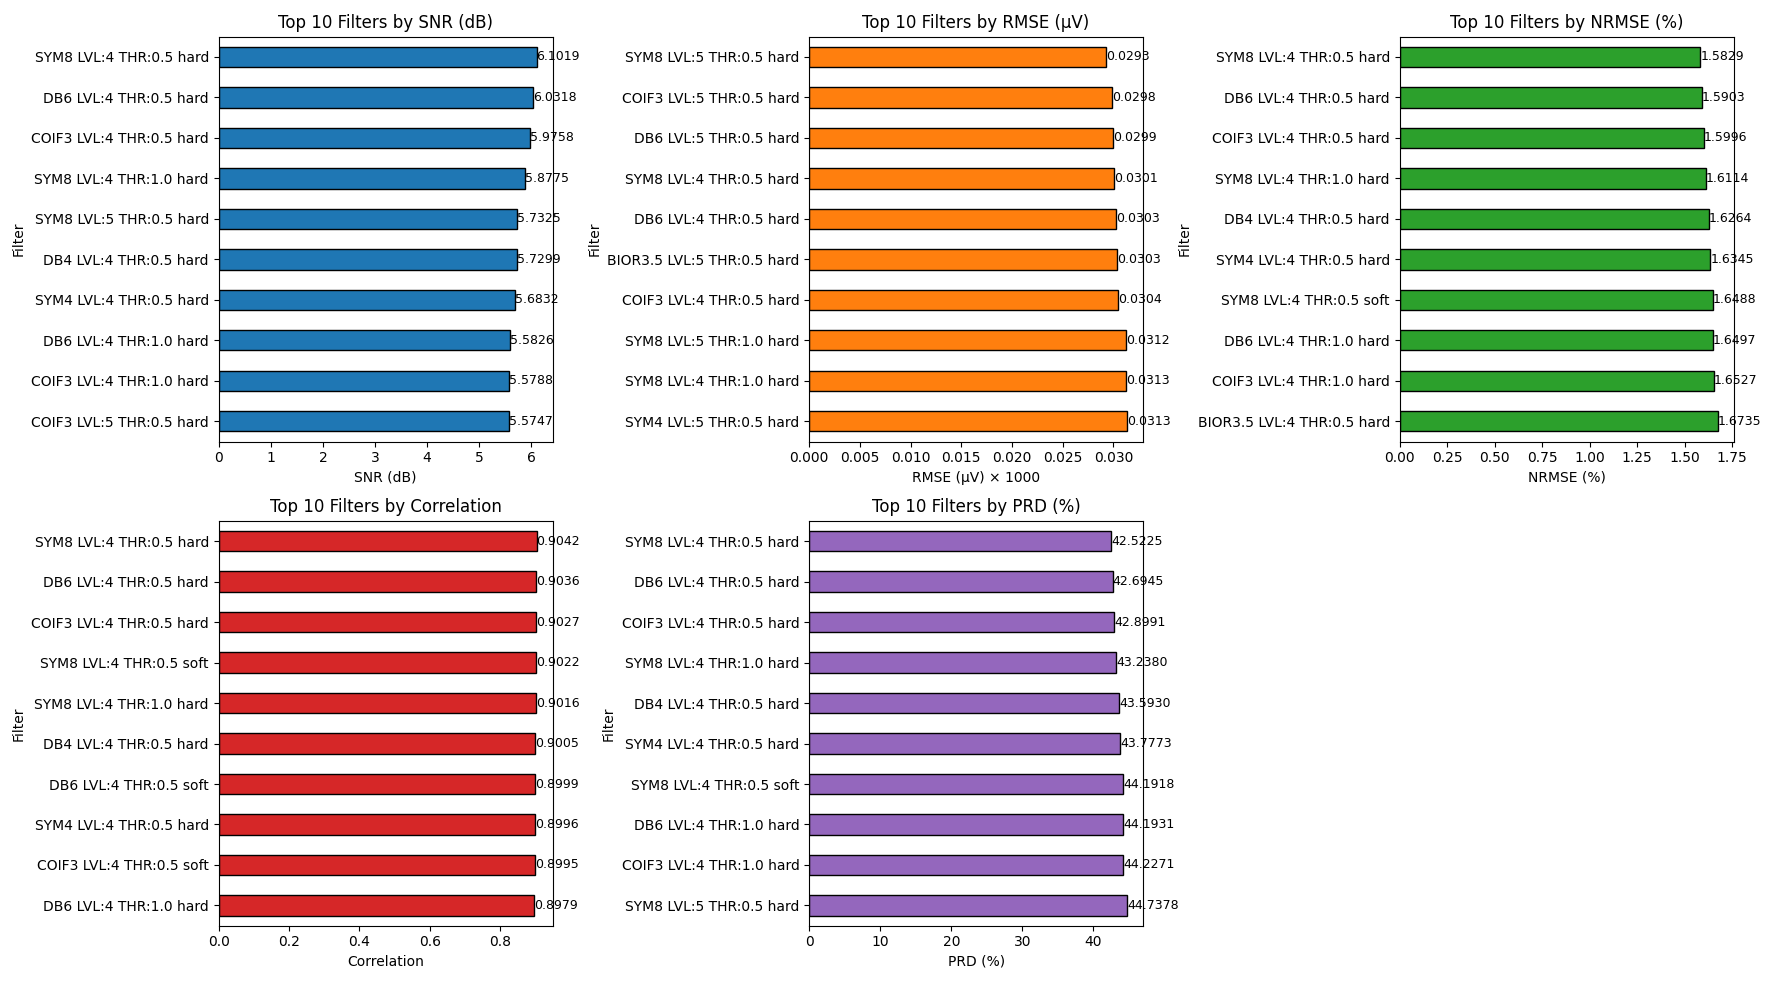
\includegraphics[width=1.1\textwidth]{eeg_metrics_result.png}
			    \caption{The top 10 filter configurations per EEG metric. RMSE values scaled.}
			    \label{}
			\end{figure}

			
			In the following figures we present a visualization using the recording named \textit{chb01\_03.edf}
			comparing the original 10 first EEG channels against the filtered ones with the respective wavelets filters.

			\begin{figure}[H]
			    \centering
			    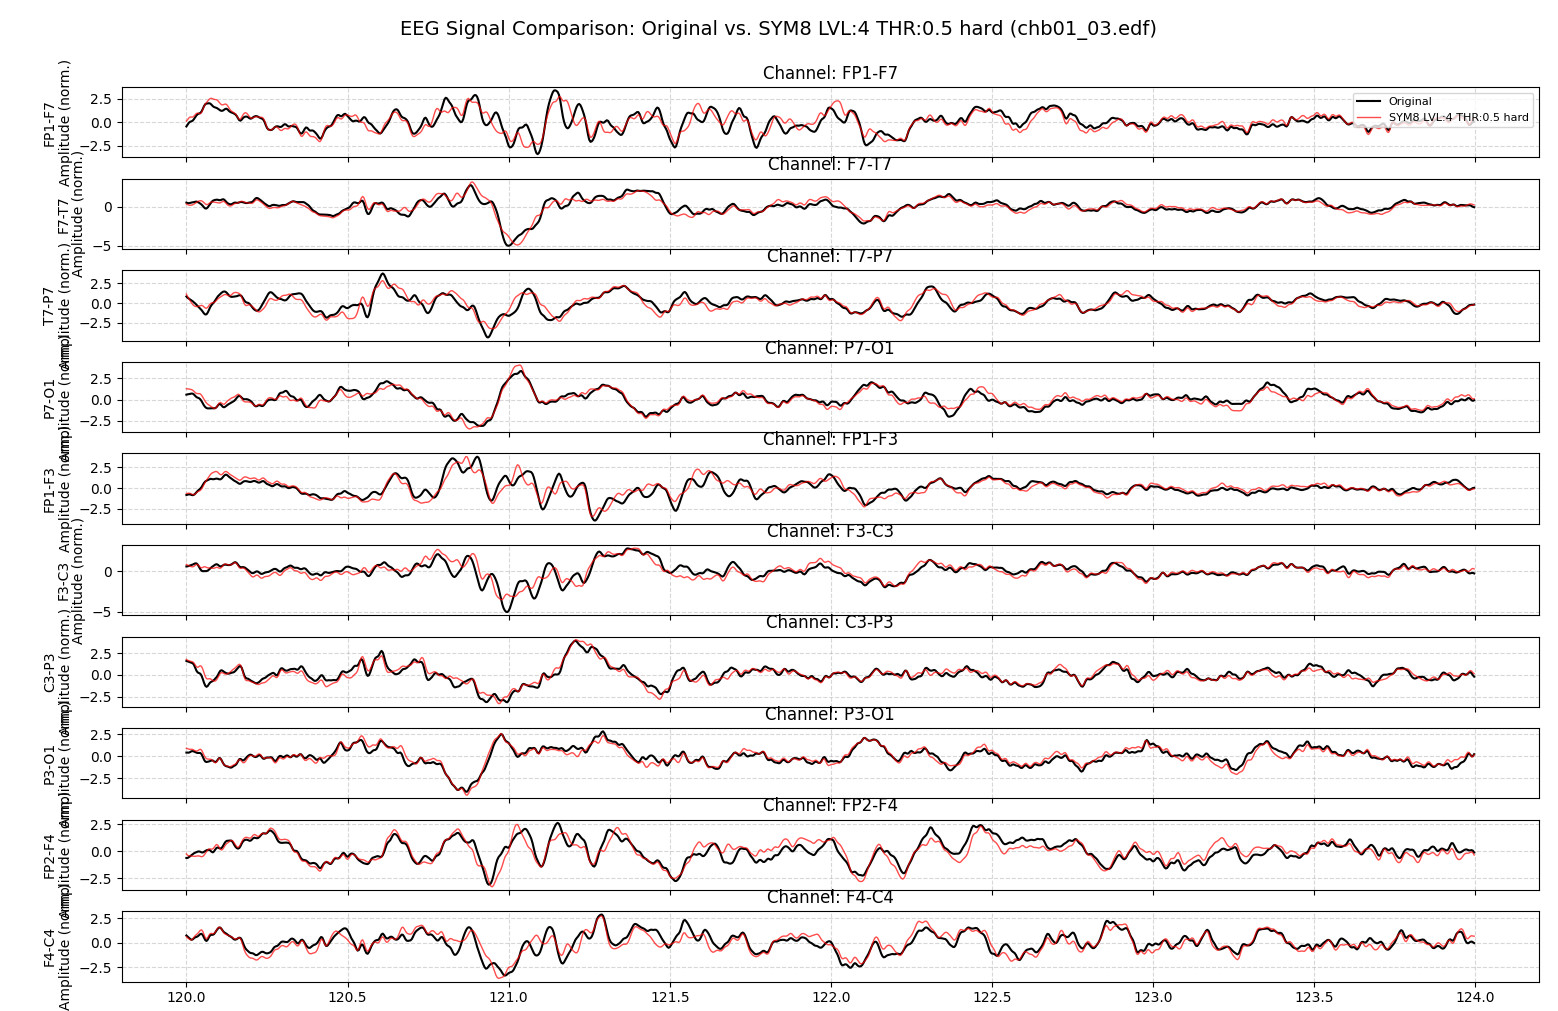
\includegraphics[width=1.2\textwidth]{wav1.png}
			    \caption{}
			    \label{}
			\end{figure}


			\begin{figure}[H]
			    \centering
			    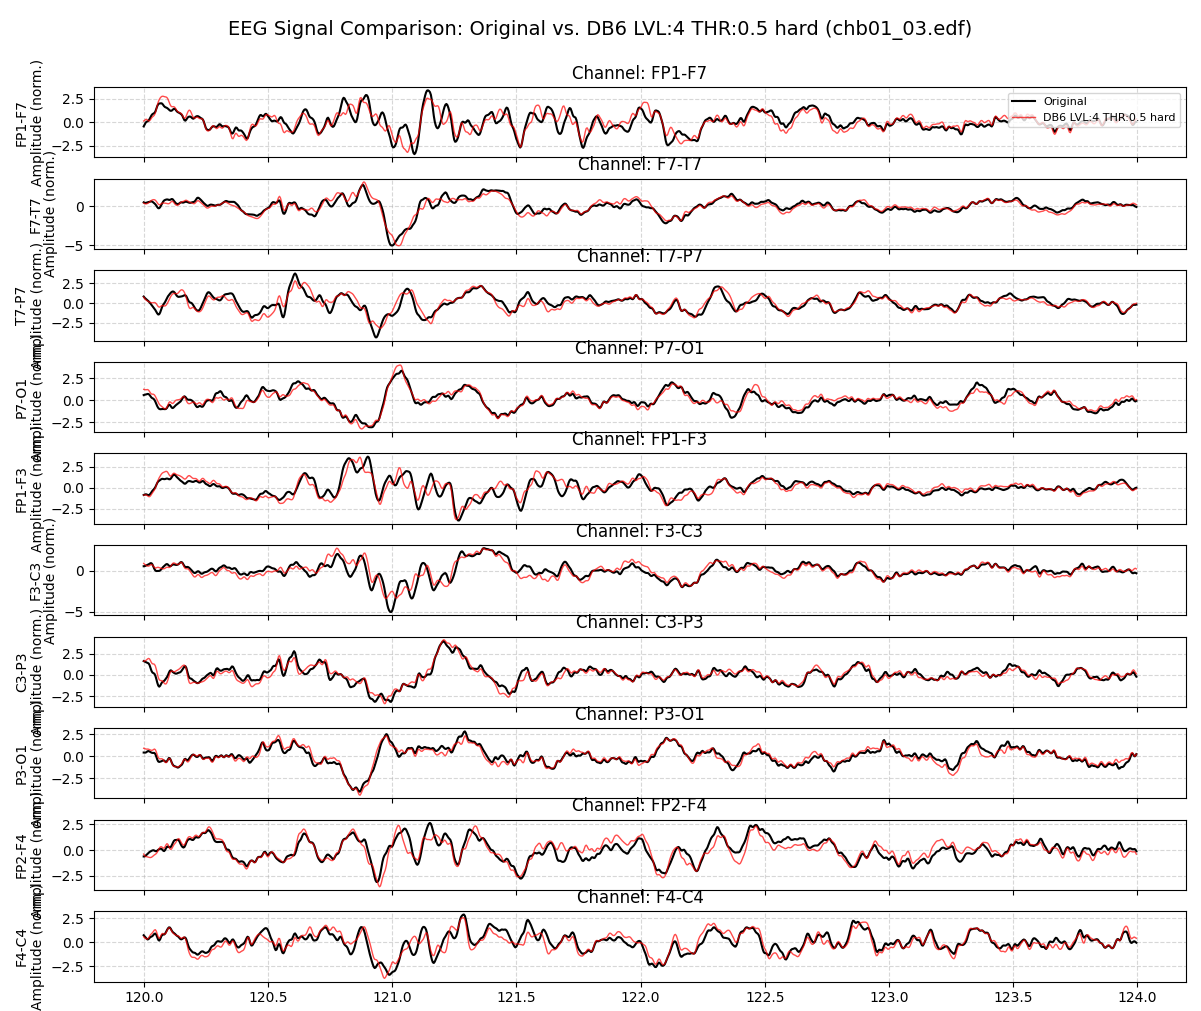
\includegraphics[width=1.2\textwidth]{wav2.png}
			    \caption{}
			    \label{}
			\end{figure}

\begin{comment}
			\begin{figure}[h]
			    \centering
			    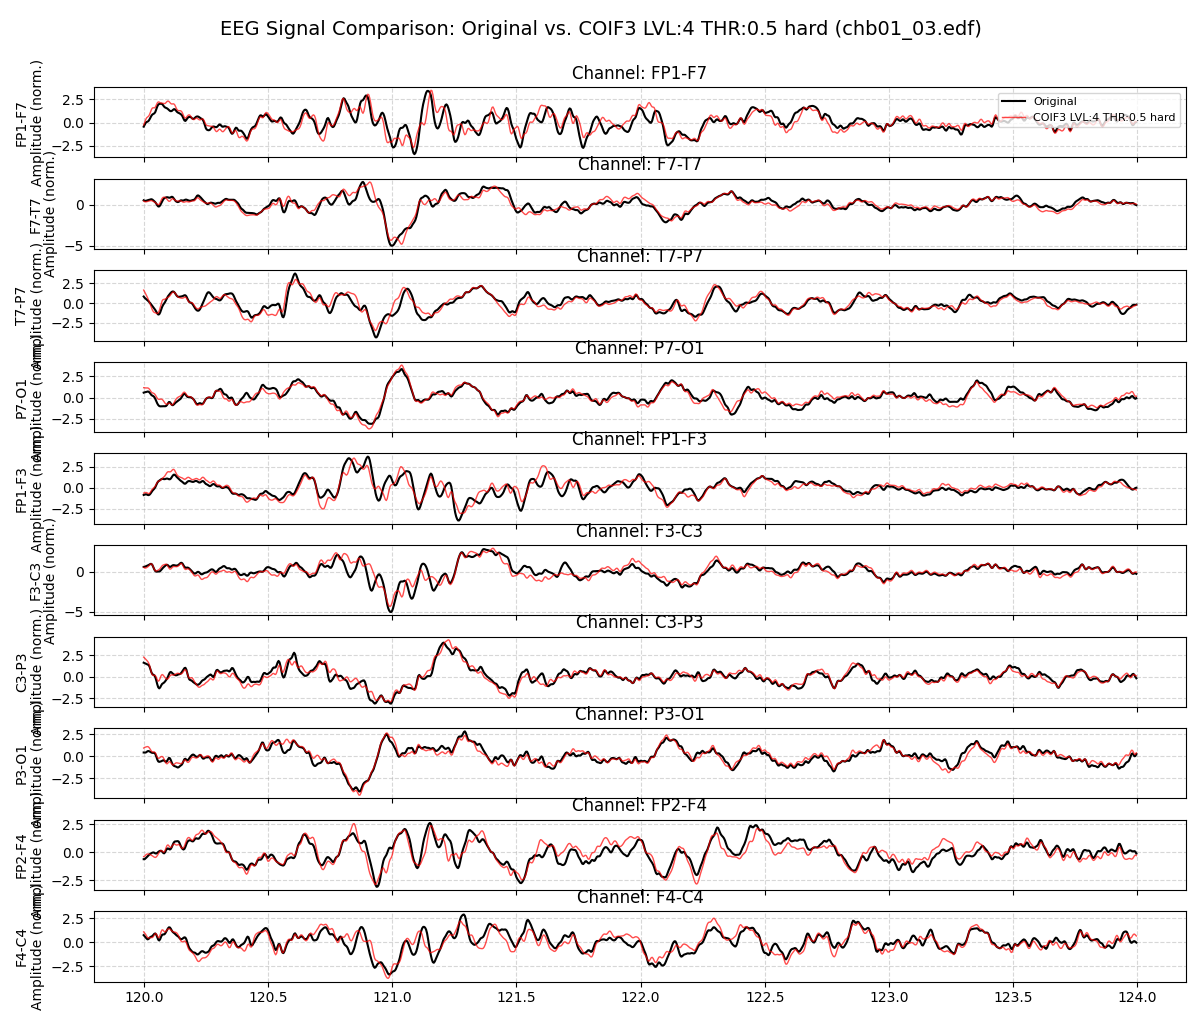
\includegraphics[width=1.2\textwidth]{wav3.png}
			    \caption{}
			    \label{}
			\end{figure}


			\begin{figure}[h]
			    \centering
			    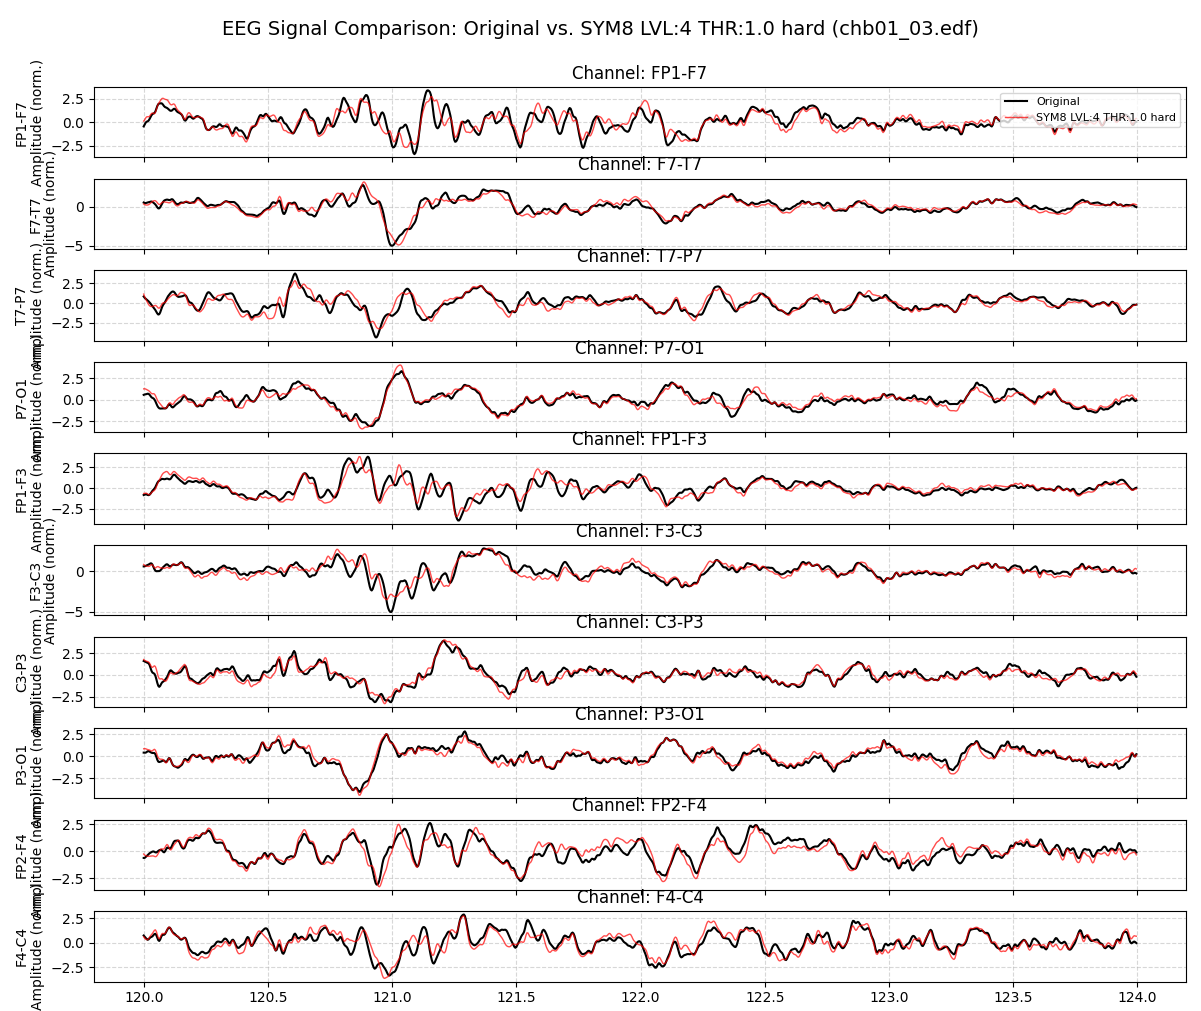
\includegraphics[width=1.2\textwidth]{wav4.png}
			    \caption{}
			    \label{}
			\end{figure}

			\begin{figure}[h]
			    \centering
			    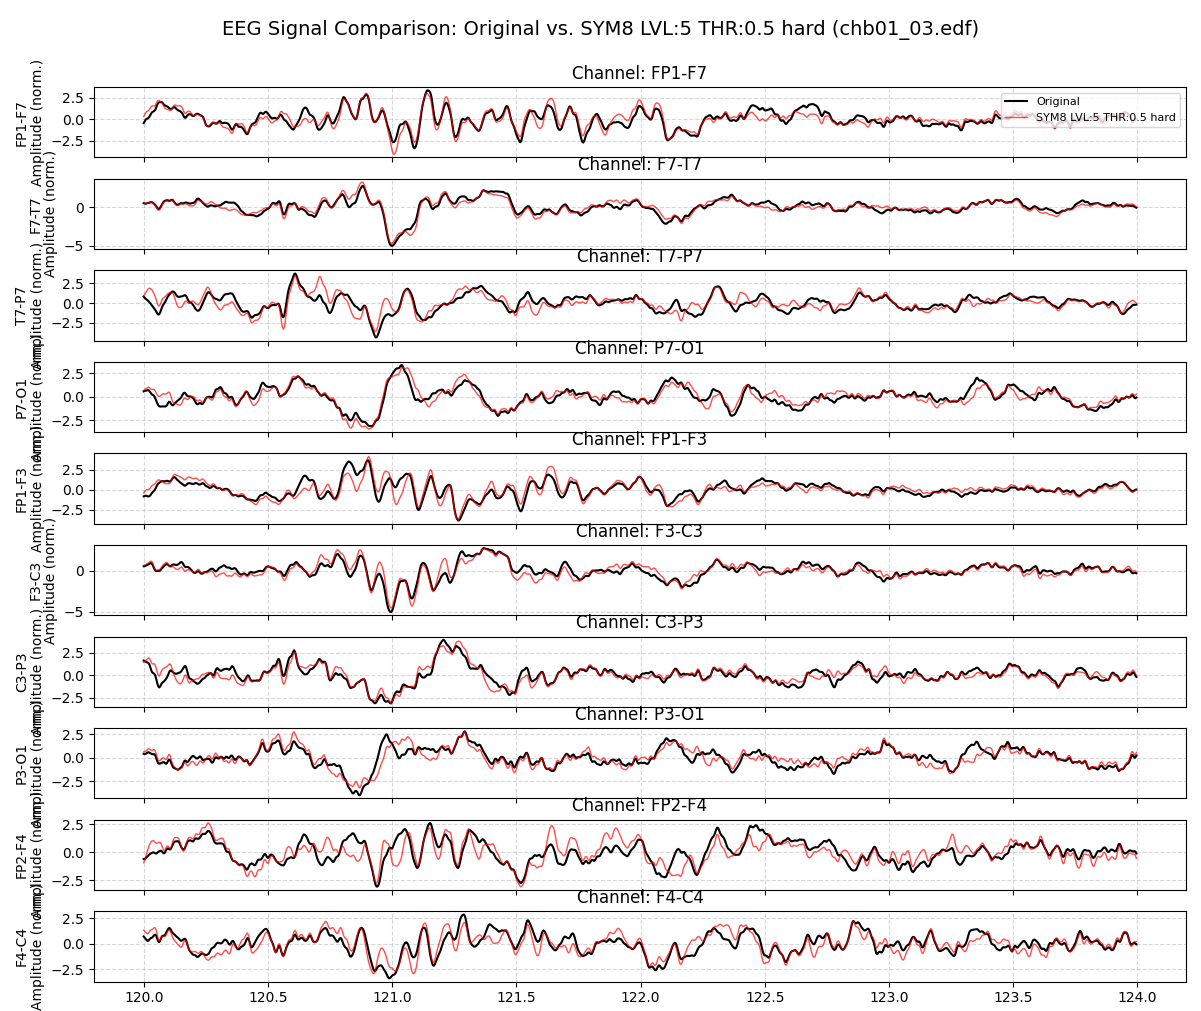
\includegraphics[width=1.2\textwidth]{wav5.png}
			    \caption{}
			    \label{}
			\end{figure}
\end{comment}

	\newpage

		\section{Phase space reconstruction of EEG signals}



		\subsection{Determination of Embedding Parameters}
		The reconstruction of the phase space from a single time series 
		\( x(t) \) requires the specification of two parameters: 
		the time delay \( \tau \) and the embedding dimension \( m \). 
		These two parameters determine how the reconstruction will represent
		and how close reveals the underlying dynamics without distortion.

		\subsubsection{Calculation of time delay \( \tau \) utilizing mutual information}
			The time delay \( \tau \) can be estimated by applying the 
			\textit{Average Mutual Information} (AMI) method, a concept which was first introduced 
			by Fraser and Swinney~\cite{fraser1986independent}. 
			In contrast to linear autocorrelation, 
			mutual information has the ability to capture both linear and nonlinear dependencies among
			the original time series \( x(t) \) and its delayed version \( x(t + \tau) \).

			The mutual information \( I(\tau) \) between \( x(t) \) and \( x(t + \tau) \) is defined as:
			\[
			I(\tau) = \sum_{x(t),\, x(t+\tau)} P(x(t), x(t+\tau)) \, \log_2 \left( \frac{P(x(t), x(t+\tau))}{P(x(t)) \, P(x(t+\tau))} \right)
			\]
			where \( P(\cdot) \) denotes probability.

			The optimal time delay \( \tau \) is chosen as the value at which 
			\( I(\tau) \) reaches its \textit{first minimum}. 
			This value indicates a good compromise 
			between independence (too small \( \tau \)) and irrelevance (too large \( \tau \)) 
			of the coordinates in the embedding vector.

			\subsubsection{Estimating embedding dimension \( m \) using false nearest neighbors approach}

			The analysis of nonlinear dynamical systems from experimental time series, such as EEG recordings, requires 
			the reconstruction of the underlying phase space from the scalar measurements of each channel. 
			According to Takens' embedding theorem \cite{takens1981}, a time series $x(t)$ can be embedded 
			in an $m$-dimensional space using time-delay coordinates:

			\begin{equation}
			\vec{y}(t) = \left[x(t), x(t+\tau), x(t+2\tau), \ldots, x(t+(m-1)\tau)\right]
			\end{equation}

			where $m$ is the embedding dimension and $\tau$ is the time delay. The critical challenge lies in determining the appropriate values for these parameters to faithfully reconstruct the system's dynamics without distortion.


			When the embedding dimension $m$ is too small, 
			the phase space becomes \emph{projected} rather than 
			properly \emph{embedded}. 
			This projection can create artificial neighborhoods where points appear to be close due to 
			geometrical constraints of the space rather than their actual dynamical similarity. 
			These are named as \emph{false nearest neighbors} \cite{kennel1992}.

			\begin{figure}[h]
			\centering
			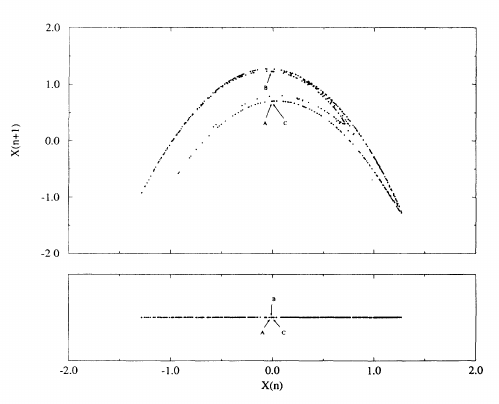
\includegraphics[width=0.8\textwidth]{fnn_schematic.png}
			\caption{Schematic illustration of false neighbors. In insufficient embedding dimension (down), points A and B appear neighbors due to projection. When proper embedding is employed(up), their true separation is revealed.}
			\label{fig:fnn_schematic}
			\end{figure}

			Mathematically, two points $\vec{y}_i$ and $\vec{y}_j$ are false neighbors if their distance increases significantly when embedded in higher dimension:

			\begin{equation}
			\frac{\|\vec{y}_i^{(m+1)} - \vec{y}_j^{(m+1)}\|}{\|\vec{y}_i^{(m)} - \vec{y}_j^{(m)}\|} > R_{\text{tol}}
			\end{equation}

			where $R_{\text{tol}}$ is a tolerance threshold (typically 10--15).

			\subsection*{The False Nearest Neighbors Algorithm}

			The FNN method \cite{kennel1992} provides a systematic approach to determine the minimal sufficient embedding dimension:

			\begin{enumerate}
			\item For each point in dimension $m$, identify its nearest neighbor
			\item Embed the data in dimension $m+1$
			\item Calculate the relative distance increase between each point and its former neighbor
			\item If the increase exceeds predetermined thresholds, classify as false neighbors
			\item The optimal $m$ is the smallest dimension where the fraction of false neighbors drops below an acceptable level (typically 1--5\%)
			\end{enumerate}

			The algorithm employs both relative and absolute criteria:

			\begin{align}
			\text{Relative:} &\quad \frac{\|\vec{y}_i^{(m+1)} - \vec{y}_j^{(m+1)}\|}{\|\vec{y}_i^{(m)} - \vec{y}_j^{(m)}\|} > R_{\text{tol}} \\
			\text{Absolute:} &\quad \|\vec{y}_i^{(m+1)} - \vec{y}_j^{(m+1)}\| > A_{\text{tol}} \cdot \sigma_x
			\end{align}

			where $\sigma_x$ is the standard deviation of the time series.

			\subsection*{Application to EEG Analysis}

			The application of FNN to EEG data is particularly important for several reasons:

			\begin{itemize}
			\item \textbf{Nonstationarity}: EEG signals exhibit nonstationary characteristics, making fixed embedding parameters suboptimal
			\item \textbf{Noise contamination}: Experimental EEG contains measurement noise and artifacts that can distort phase space reconstruction
			\item \textbf{Subject variability}: Optimal embedding may vary across subjects, brain states, and recording conditions
			\item \textbf{Computational efficiency}: FNN provides a data-driven approach that adapts to individual recordings
			\end{itemize}
					
	\newpage

\bibliographystyle{plain}
\bibliography{references}

\end{document}
